
\documentclass[a4paper,12pt]{scrbook}
\usepackage{amsmath,amssymb,amsthm}
\usepackage{fancyvrb}
\usepackage{parskip}
\usepackage{lastpage}
\usepackage{verbatim,boxedminipage,enumitem}
\usepackage{ifthen}
\usepackage{color,graphicx}
\usepackage{pgf}
\usepackage{longtable}
\usepackage{upquote}
%\usepackage[all]{xy}
\usepackage{tobiShell}
\usepackage{tikz}
\usetikzlibrary{automata}
\usetikzlibrary{arrows}
\usepackage{pgf,pgfarrows,pgfnodes}
\usepackage{pgfplots}
\usepackage{circuitikz}
\usetikzlibrary{circuits}
\usetikzlibrary{circuits.logic.US}
\usepackage{mymath}
\usepackage{python}
%------------------------------------------------------------------
% Verbatim for console window - single line frame, no line numbers
%------------------------------------------------------------------
\DefineVerbatimEnvironment%
 {console}{Verbatim}
 {frame=single}

%--------------------------------------------------------
% Remove the vertical spacing before and after Verbatim.
%--------------------------------------------------------
\usepackage{atbeginend}
\BeforeBegin{console}{\mbox{}\\ \begin{minipage}{\textwidth}\vspace{3pt}}
\AfterEnd{console}{\vspace{4pt} \end{minipage} \\ }

\begin{document}
\thispagestyle{empty}

\begin{center}
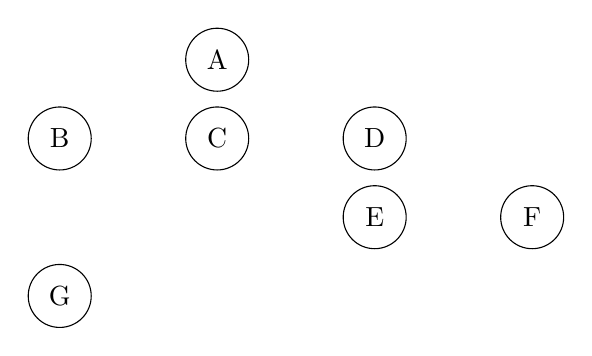
\begin{tikzpicture}

\draw[black] (2.0, 0.0)
circle (0.4);
\draw (2.0, 0.0) node[color=black] {A};
\draw[black] (2.0, -1.0)
circle (0.4);
\draw (2.0, -1.0) node[color=black] {C};
\draw[black] (0.0, -1.0)
circle (0.4);
\draw (0.0, -1.0) node[color=black] {B};
\draw[black] (4.0, -2.0)
circle (0.4);
\draw (4.0, -2.0) node[color=black] {E};
\draw[black] (4.0, -1.0)
circle (0.4);
\draw (4.0, -1.0) node[color=black] {D};
\draw[black] (0.0, -3.0)
circle (0.4);
\draw (0.0, -3.0) node[color=black] {G};
\draw[black] (6.0, -2.0)
circle (0.4);
\draw (6.0, -2.0) node[color=black] {F};
\end{tikzpicture}

\end{center}

\end{document}
